
\section{Raspberry Pi}

\begin{frame}
\frametitle{Raspberry Pi}

\begin{center}
  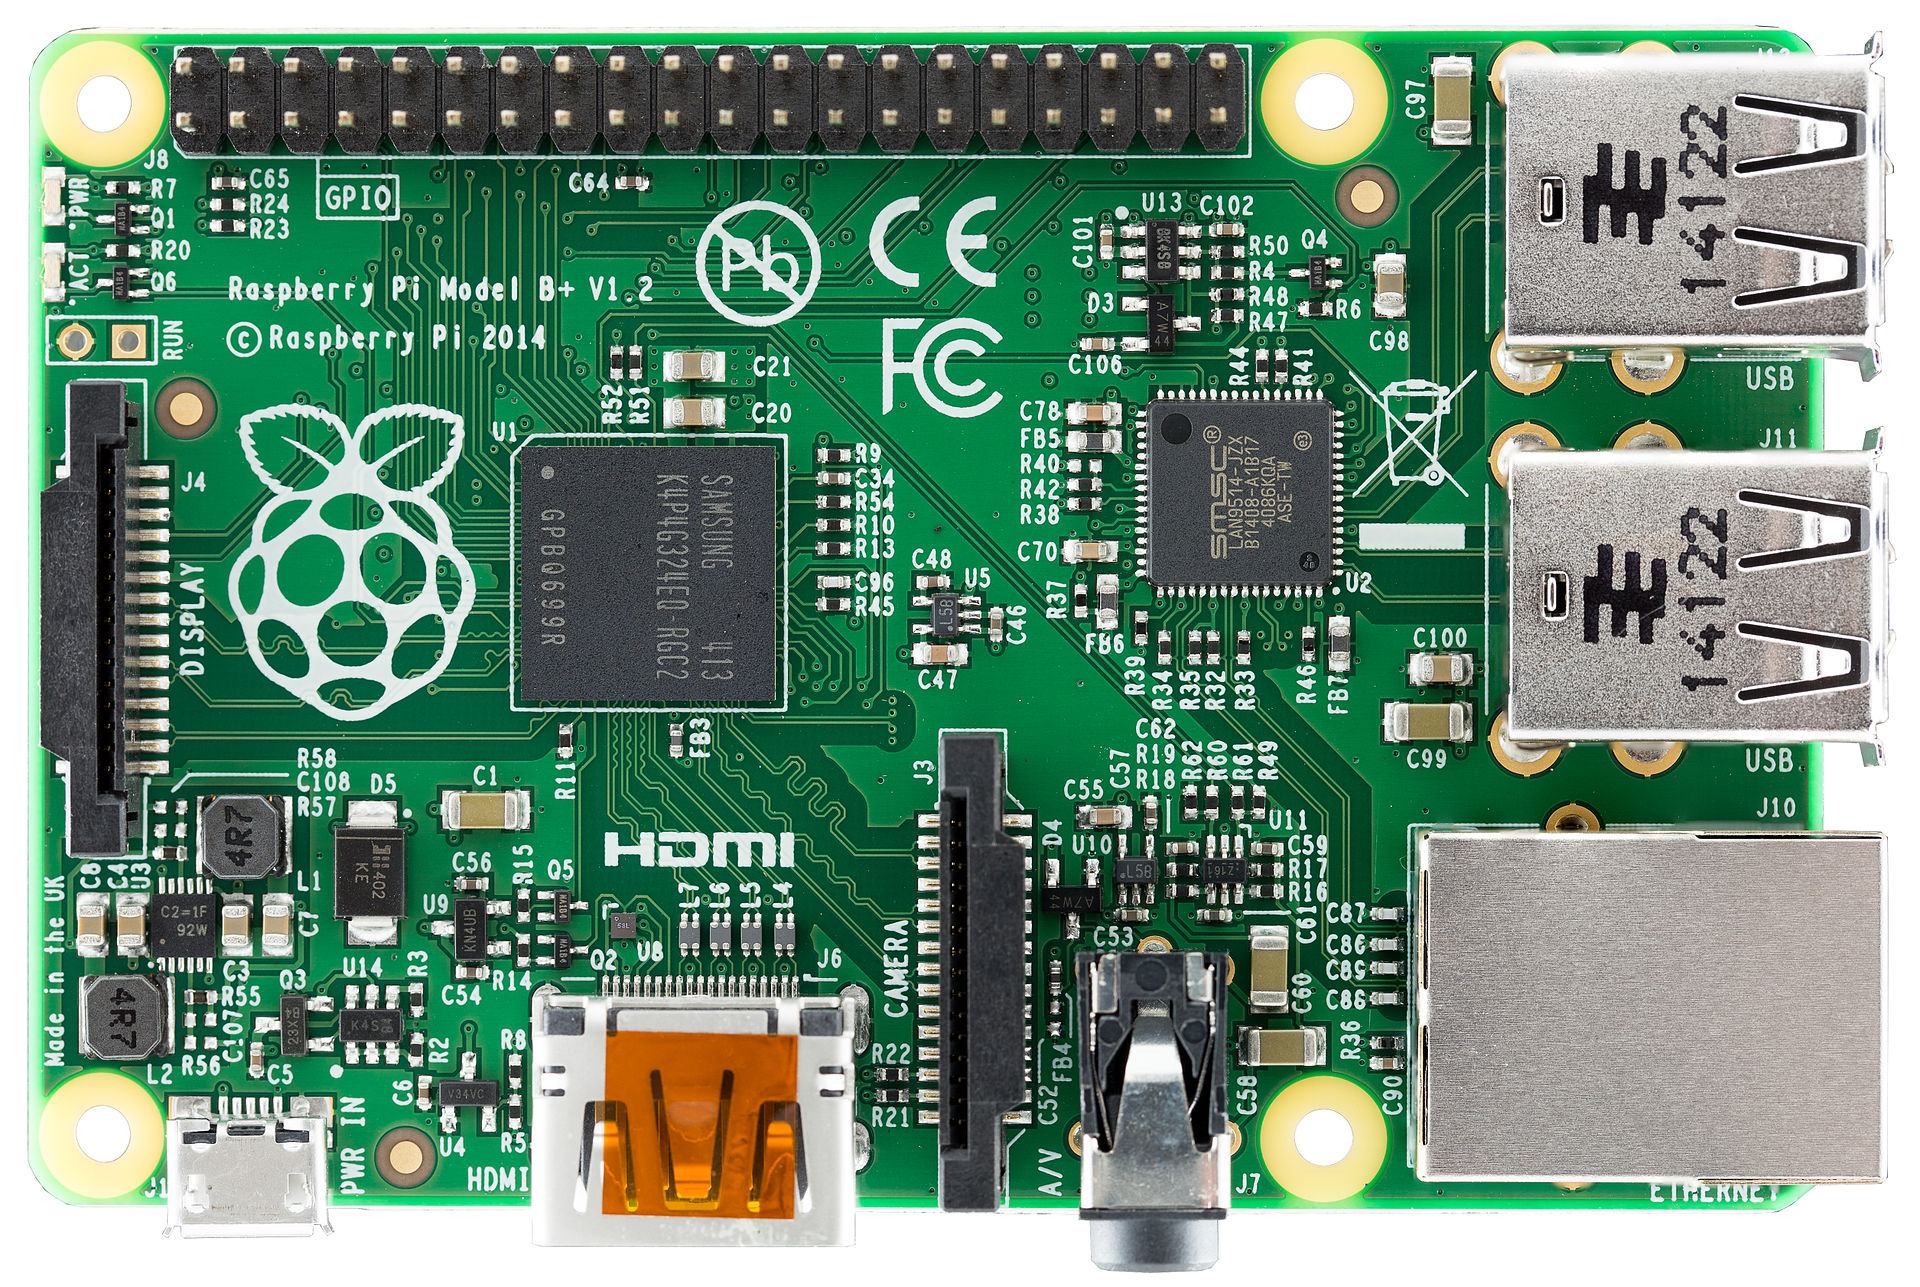
\includegraphics[width=10cm]{figs/raspberry.jpg}
\end{center}


\begin{flushright}
{\tiny
Source: Wikipedia
}
\end{flushright}

\end{frame}

%-----------------------    ---------------------------------

\begin{frame}
\frametitle{¿Qué es la Raspberry Pi?}

\begin{itemize}
   \item Ideada para educación; para entender cómo funciona la computación
   \item Es una placa de ordenador del tamaño de una tarjeta de crédito
   \item Cuesta 35 euros (sólo la placa)
   \item Muchos accesorios (incluidas cajas)
   \item Cuenta con sistemas operativos específicos
   \item El sistema operativo va en una tarjeta microSD
   \item Muchos proyectos \emph{maker}: sistema multimedia casero, servidor web,
\emph{router}, y muchos más.
\end{itemize}

\end{frame}


%-----------------------    ---------------------------------

\begin{frame}
\frametitle{Raspberry Pi: Puertos}

\begin{center}
  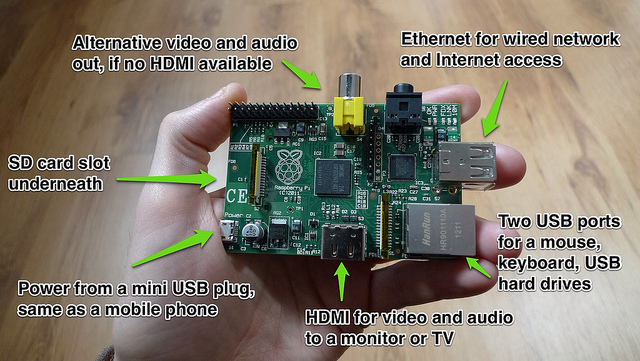
\includegraphics[width=11cm]{figs/raspberry2.jpg}
\end{center}


\begin{flushright}
{\tiny
(cc) Phil Sheard (from Flickr)
}
\end{flushright}

\end{frame}


